
% ************* PREAMBLE

\documentclass{beamer}

% ------------- THEME

\usetheme[block=fill]{metropolis}
\usepackage{appendixnumberbeamer}
\usepackage{booktabs}
\usepackage[scale=2]{ccicons}
\usepackage{pgfplots}
\usepgfplotslibrary{dateplot}
\usepackage{xspace}
\newcommand{\themename}{\textbf{\textsc{metropolis}}\xspace}

% ------------- REFERENCES

\usepackage[backend=biber,style=apa]{biblatex}
\addbibresource{references.bib}

% ------------- COLOR

\usepackage{xcolor}
\definecolor{lightgray}{RGB}{211, 211, 211}

% ------------- OTHER PACKAGES

\usepackage[italian]{babel}
\usepackage[utf8]{inputenc}

\usepackage{stmaryrd}

\usepackage{amssymb}
\usepackage{amsmath}
\usepackage{latexsym}
\usepackage{amsthm}
\usepackage{mathabx}

\usepackage{hyperref}
\usepackage{caption}

% ------------- GENERAL INFORMATION

\title{Towards a Categorical Foundation of Deep Learning: A Survey}
\subtitle{Una rassegna di approcci categorici al \textit{deep learning}}
\author{Francesco Riccardo Crescenzi}
\institute{Alma mater studiorum - Università di Bologna \\ CdL in Matematica}


% ************* DOCUMENT

\begin{document}

\maketitle

\begin{frame}[standout]
    \Huge We are in an AI summer, but is winter coming?
\end{frame}
\begin{frame}{Problemi con il deep learning}
    \large Mancano fondamenta teoriche:
    \begin{itemize}
        \item<1-> \textbf{design ad hoc} {\footnotesize(\cite{gavranovic2024fundamental})}
        \item<2-> \textbf{complessità fine a se stessa} {\footnotesize(\cite{rahimi2017machine})}
        \item<3-> \textbf{fragilità} {\footnotesize(\cite{gavranovic2024fundamental})}
    \end{itemize}
\end{frame}

\begin{frame}{Problemi con il deep learning}
    \large La ricerca viene rallentata da:
    \begin{itemize}
        \item<1-> \textbf{research debt} {\footnotesize(\cite{olah2017research})}
        \item<2-> \textbf{mancata replicabilità} {\footnotesize(\cite{raff2019step})}
    \end{itemize}
\end{frame}

\begin{frame}[standout]
    \centering \Huge Teoria delle categorie: \\\large una lingua franca della matematica e delle scienze
\end{frame}

\begin{frame}{Teoria delle categorie applicata}
    \centering La teoria delle categorie studia strutture e relazioni, e può essere vista come un'estensione del celebre \textit{Erlangen Programme}.

    \centering La teoria delle categorie può essere applicata con successo anche in fisica, informatica, chimica... ovunque ci sia \textbf{composizionalità} (\cite{fong2018seven}).
\end{frame}

\begin{frame}{Teoria delle categorie applicata}
    \begin{itemize}
        \item<1-> \textbf{lenti parametriche} {\footnotesize (\cite{gavranovic2024fundamental}, \cite{cruttwell2022categorical})}
        \item \textbf{categorical deep learning}{\footnotesize(\cite{gavranovicposition})}
        \item \textbf{integral transforms} {\footnotesize(\cite{dudzik2022graph}, \cite{dudzik2024asynchronous})}
        \item \textbf{functor learning} {\footnotesize(\cite{gavranovic2019compositional}, \cite{sheshmani2021categorical}, \cite{chytas2024poolingimagedatasetsmultiple})}
        \item \textbf{compositional distributional model of meaning} {\footnotesize(\cite{clark2007combining}, \cite{coecke2010mathematical}, \cite{lewis2019compositionality})}
        \item \textbf{neural circuit diagrams} {\footnotesize(\cite{abbott2023robust})}
        \item \textbf{string diagrams with universal approximators} {\footnotesize(\cite{khatri2024anatomy})}
    \end{itemize}
\end{frame}

\begin{frame}{Teoria delle categorie applicata}
    \begin{itemize}
        \item \textbf{lenti parametriche} 
        \item \textbf{categorical deep learning} 
        \item \textcolor{lightgray}{\textbf{integral transforms}}
        \item \textcolor{lightgray}{\textbf{functor learning}} 
        \item \textcolor{lightgray}{\textbf{compositional distributional model of meaning}}
        \item \textcolor{lightgray}{\textbf{neural circuit diagrams}}
        \item \textcolor{lightgray}{\textbf{string diagrams with universal approximators}}
    \end{itemize}
\end{frame}


\begin{frame}[standout]
    \huge Lenti parametriche \\\large per modellare il gradient-based learning
\end{frame}

\begin{frame}{Gradient-based learning con lenti parametriche}
    Il gradient-based learning segue tre principi fondamentali:
    \begin{itemize}
        \item<1-> \textbf{parametricità}
        \item<2-> \textbf{bidirezionalità}
        \item<3-> \textbf{differenziabilità}
    \end{itemize}
\end{frame}

\begin{frame}{Gradient-based learning con lenti parametriche}
    \begin{block}{DEFINIZIONE: Il costrutto $\mathbf{Para}$}
        Sia $(\mathcal{C},I,\otimes)$ una categoria monoidale strettamente simmetrica. Allora, $\mathbf{Para}_{\otimes}(\mathcal{C})$ è la $2$-categoria definita come segue.
        \begin{itemize}
          \item Le $0$-celle sono oggetti di $\mathcal{C}$.
          \item Le $1$-cells sono coppie $(P,f): A \to B$, dove $P : \mathcal{C}$ e $f: P \otimes A \to B$.
          \item The $2$-celle sono $r: (P,f) \Rightarrow (Q,g)$, dove $r: P \to Q$ è un morfismo in $\mathcal{C}$ che rispetta certe condizioni di naturalità.
        \end{itemize}
        Vedasi \cite{gavranovic2024fundamental}.
      \end{block}
\end{frame}

\begin{frame}{Gradient-based learning con lenti parametriche}
    \begin{figure}
        \begin{center}
            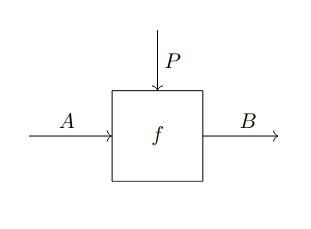
\includegraphics[width=0.5\textwidth]{figures/para.png}
            \caption*{\cite{gavranovic2024fundamental}}
        \end{center}
    \end{figure}
\end{frame}

\begin{frame}{Gradient-based learning con lenti parametriche}
    \begin{block}{DEFINIZIONE: Il costrutto $\mathbf{Lens}$}
        Sia $(\mathcal{C},1,\times)$ una categoria Cartesiana. Allora, $\mathbf{Lens}(\mathcal{C})$ è la categoria definita come segue.
        \begin{itemize}
          \item Un oggetto di $\mathbf{Lens}(\mathcal{C})$ è una coppia $\left(\begin{smallmatrix} A \\ A' \end{smallmatrix}\right)$ di oggetti di $\mathcal{C}$.
          
          \item Un morfismo $\left(\begin{smallmatrix} A \\ A' \end{smallmatrix}\right) \to \left(\begin{smallmatrix} B \\ B' \end{smallmatrix}\right)$ (anche chiamato lente) è una coppia $\left(\begin{smallmatrix} f \\ f' \end{smallmatrix}\right)$ di morfismi di $\mathcal{C}$ tali che $f: A \to B$ and $f': A \times B' \to A'$. La mappa $f$ è nota come \textit{forward pass} della lente, mentre la mappa $f'$ è nota come \textit{backward pass}.
        \end{itemize}
        Vedasi \cite{cruttwell2022categorical}.
      \end{block}
\end{frame}

\begin{frame}{Gradient-based learning con lenti parametriche}
    \begin{figure}
        \begin{center}
            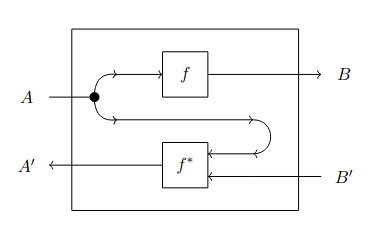
\includegraphics[width=0.7\textwidth]{figures/lens_inner_view.png}
            \caption*{\cite{cruttwell2022categorical}}
        \end{center}
    \end{figure}
\end{frame}

\begin{frame}{Gradient-based learning con lenti parametriche}
    \begin{block}{DEFINIZIONE: Cartesian reverse differential category}
        Una \textit{Cartesian reverse differential category} (CRDC) $\mathcal{C}$ è una categoria Cartesiana con una struttura additiva dove è definito un operatore differenziale $\mathrm{R}$ che ha le proprietà di una \textit{reverse derivative}.
        Si vedano \cite{cockett2019reverse} e \cite{gavranovic2024fundamental}.
      \end{block}

      \begin{block}{ESEMPIO: $\mathbf{Smooth}$}
        Consideriamo $\mathbf{Smooth}$, ovvero la categoria degli spazi Euclidei e delle funzioni liscie. $\mathbf{Smooth}$ è una CRDC rispetto all'operatore
        \[\mathrm{R}[f]: (x,y) \mapsto \mathcal{J}_f(x)^Ty.\]
      \end{block}
\end{frame}

\begin{frame}{Gradient-based learning con lenti parametriche}
    \begin{figure}
        \begin{center}
            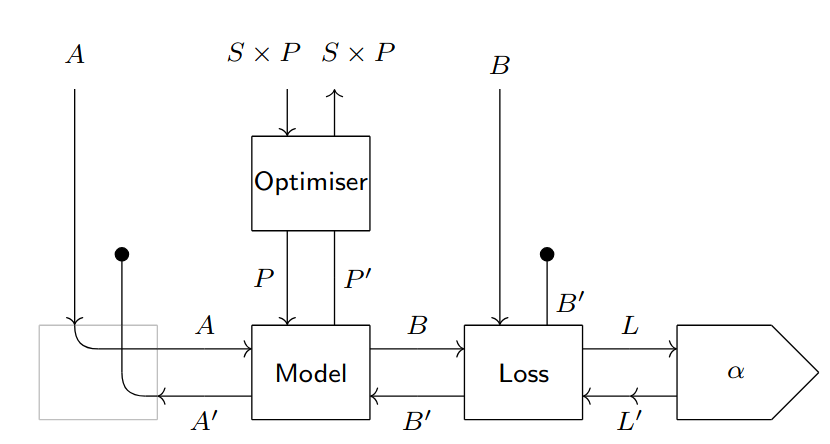
\includegraphics[width=\textwidth]{figures/lenses_supervised_learning2.png}
            \caption*{\cite{cruttwell2022categorical}}
        \end{center}
    \end{figure}
\end{frame}

\begin{frame}[standout]
    \huge Categorical deep learning: \\\large (co)algebre categoriche \\come teoria delle architetture
\end{frame}

\begin{frame}{Dal GDL al CDL}
    \begin{block}{\textit{Geometric deep learning}}
        Il \textit{geometric deep learning} è una teoria delle architetture di reti neurali che imita l'\textit{Erlangen Programme}, organizzando le architetture in base al concetto di equivarianza rispetto ad azioni di gruppi (\cite{bronstein2021geometric}).
    \end{block}
\end{frame}

\begin{frame}{Dal GDL al CDL}
    \begin{block}{\textit{Categorical deep learning}}
        Il \textit{categorical deep learning} è una teoria delle architetture di reti neurali che generalizza il GDL, organizzando le architetture in base al concetto di omomorfismo di (co)algebre categoriche (\cite{gavranovicposition}).
    \end{block}
\end{frame}


\begin{frame}{Dal GDL al CDL}
    \begin{block}{DEFINIZIONE: Algebra su un endofuntore}
        Sia $F: \mathcal{C} \to \mathcal{C}$ un endofuntore. Un'algebra su $F$ è una coppia $(A,a)$ dove $A$ è un oggetto di $\mathcal{C}$ e $a: F(A) \to A$ è un morfismo in $\mathcal{C}$.
    \end{block}

    \begin{block}{DEFINIZIONE: Omomorfismo di algebre}
        Siano $(A,a)$ e $(B,b)$ algebre sollo stesso endofuntore $F: \mathcal{C} \to \mathcal{C}$. Un omomorfismo di algebre $(A,a) \to (B,b)$ è un morfismo $f: A \to B$ in $\mathcal{C}$ tale che $F(f) \fatsemi b =  a \fatsemi f$.
    \end{block}
\end{frame}

\begin{frame}{Dal GDL al CDL}
    \begin{figure}
        \begin{center}
            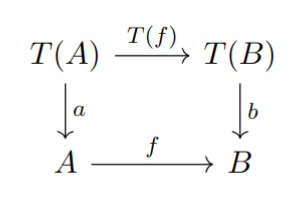
\includegraphics[width=0.5\textwidth]{figures/algebra_hom.png}
            \caption*{}
        \end{center}
    \end{figure}
\end{frame}

\begin{frame}{Dal GDL al CDL}
    \begin{block}{ESEMPIO: Liste}
        Sia $A$ un insieme. Consideriamo l'endofuntore $1 + A \times -$ su $\mathbf{Set}$. Sia $\mathsf{List}(A)$ l'insieme delle liste di elementi di $A$. Allora, se $\mathsf{Nil}: 1 \to {List}(A)$ mappa l'unico oggetto di $1$ alla lista vuota e $\mathsf{Cons}: A \times \mathsf{List}(A) \to \mathsf{List}(A)$ aggiunge un elemento a una lista, $(\mathsf{List}(A), [\mathsf{Nil}, \mathsf{Cons}])$, è un algebra su $1 + A \times -$. (Esempio da \cite{gavranovicposition}.)
    \end{block}
\end{frame}

\begin{frame}{Dal GDL al CDL}
    \begin{block}{ESEMPIO: \textit{List folds}}
        Consideriamo due algebre $(\mathsf{List}(A), [\mathsf{Nil}, \mathsf{Cons}])$ e $(Z, [r_0,r_1])$ su $1 + A \times -$. Un omomorfismo $f: \mathsf{List}(A) \to Z$ tra queste due algebre deve soddisfare 
        \begin{align*}
            f(\mathsf{Nil}) &= r_0,\\
            f(\mathsf{Cons}(a,l)) &= r_1(a,f(l)). 
        \end{align*}
        Hence, $f$ è necessariamente un \textit{fold} che riduce liste di elementi di $A$ a singoli elementi di $Z$. (Esempio da \cite{gavranovicposition}.)
    \end{block}
\end{frame}

\begin{frame}{Dal GDL al CDL}
    \begin{figure}
        \begin{center}
            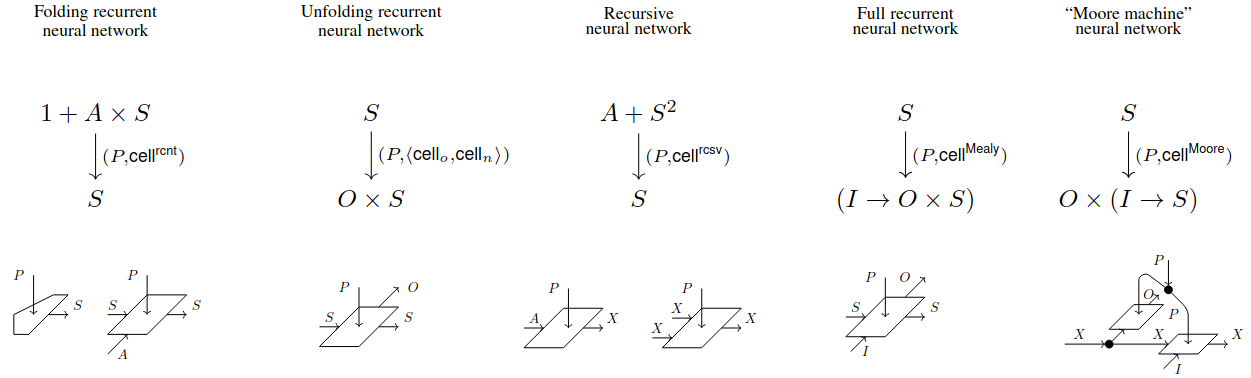
\includegraphics[width=1\textwidth]{figures/cells.png}
            \caption*{\cite{gavranovicposition}}
        \end{center}
    \end{figure}
\end{frame}


\begin{frame}[standout]
    \huge Prospettive future
\end{frame}

\begin{frame}{Prospettive future}
    C'è una competizione in corso tra varie discipline, che puntano a spiegare le reti neurali utilizzando ciascuna i propri strumenti:
    \begin{itemize}
        \item<1-> \textbf{fisica matematica} {\footnotesize (e.g. \cite{roberts2022principles})},
        \item<2-> \textbf{topologia} {\footnotesize (e.g. \cite{hensel2021survey})},
        \item<3-> \textbf{probabilità} {\footnotesize (e.g. \cite{patel2015probabilistic})},
        \item<4-> e così via...
    \end{itemize}
    
\end{frame}

\begin{frame}{Prospettive future}
    La teoria delle categorie, oltre a offrire strumenti propri, potrebbe creare un ponte tra queste discipline e potrebbe unificare i loro approcci in una teoria generale del deep learning.
\end{frame}

\begin{frame}[allowframebreaks]
    \printbibliography
\end{frame}

\end{document}